\subsection{Abstract Domains}\label{subsec:abstract-domains}

In the following section we will describe the abstract domains of our value analysis.

\subsubsection{Abstract domain of strings as regular expressions}\label{subsubsec:abstract_domains_strings}
We have chosen regular expressions/languages to represent the abstract domain of the family of SQL string data types.
Regular expressions/languages are chosen instead of more powerful representations because of the decidable nature of inclusion and equality between them.

Let $\regexs$ denote the set of regular expressions, for elements of $\regex \in \regexs$ we denote the language of $\regex$ as $\lang(\regex)$.
In general we will not distinguish between $R$ and $\lang(\regex)$ when it simplifies matters.
The lattice of $(\regexs, \subseteq, \cup, \cap)$ is a lattice but not a finite one, this is a problem: Essentially, we want the state-space our analysis to be finite, such that we can employ the Kleene fixed-point theorem (see \autoref{thm:kleene_finite}) to prove the termination of our analysis.
If the state-space is built from infinite parts the state-space itself will be infinite.
We will 'fix' this problem later in \autoref{sec:cover-lattice}.
Naturally we define the concretisation of regular expression as it's language:
\begin{align}
    \concrete_6 &: \mathbf{REG} \rightarrow \mathcal{P}(\mathbf{STR}) \\
    \concrete_6(R) &= \mathcal{L}(R)
\end{align}
Where $\strs$ denote the set of all strings.

\subsubsection{Abstract domain of integers as union intervals}\label{subsubsec:abstract_domains_numbers} We have chosen a finite union and intersection of intervals to represent the abstract domain of the family of SQL number data types.
We call them union of intervals as all such objects can be written as a union of intervals.
We only consider integers, but we imagine that the domain can be easily extended to the reals.
Let $\mathbf{INT}$ be the set of union intervals, that is inductively defined as:
\[
    \inference{i \text{ is an interval}}{i \in \mathbf{INT}} \quad
    \inference{\mathscr{I}_1 \in \textbf{INT} & \mathscr{I}_2 \in \textbf{INT}}{\mathscr{I}_1 \cup  \mathscr{I}_2 \in \mathbf{INT}} \quad
    \inference{\mathscr{I}_1 \in \textbf{INT} & \mathscr{I}_2 \in \textbf{INT}}{\mathscr{I}_1 \cap  \mathscr{I}_2 \in \mathbf{INT}}
\]

For integers we will only consider $[a, b], [a, +\infty)$ and $(-\infty, b]$ where $a, b \in \mathbb{Z}$ as valid intervals.

This abstract representation of numbers $(\uints, \subseteq, \cup, \cap)$ has the same issue as regular expressions: It is not finite.
We define the concretisation of union intervals as follows:
\begin{align}
    \concrete_6 &: \mathbf{INT} \rightarrow \mathcal{P}(\mathbf{NUM}) \\
    \concrete_6(\uint_1 \cup \uint_2) &= \concrete_6(\uint_1) \cup \concrete_6(\uint_2) \\
    \concrete_6(\uint_1 \cap \uint_2) &= \concrete_6(\uint_1) \cap \concrete_6(\uint_2) \\
    \concrete_6([a, b]) &= \left\{ z \in \mathbb{Z} \middle| a \leq z \leq b \right\} \\
    \concrete_6([a, +\infty]) &= \left\{ z \in \mathbb{Z} \middle| a \leq z \right\} \\
    \concrete_6([-\infty, b]) &= \left\{ z \in \mathbb{Z} \middle| z \leq b \right\}
\end{align}

This abstract domain is most likely not a new development, the title of \cite{li2010abstract} suggest a similar construct, but we have been unable to get a hold of their paper.

\subsubsection{Cover lattice}\label{sec:cover-lattice}
To resolve the issues presented above, we introduce the notion of a cover lattice.
As above the idea presented here is probably not novel.
Before we can define a cover lattice, we need to define the notion of a top-cover.

\begin{definition}
    A finite non-empty subset $X \subseteq S$ of a lattice $(S, \subseteq, \cup, \cap)$ is called a collectively top-cover of $S$ whenever $\bigcup X = \top$.
\end{definition}

\begin{definition}\label{def:coverlattice}
Given a collectively top-cover $X$ of a lattice $(S, \subseteq, \cup, \cap)$.
A cover lattice of $S$ in respect to $X$ denoted $\clattice{X}{S}$ is the minimum set where,
For $X$ and $S$:
\begin{align}
    \inference{x \in X}{x \in C_X(S)} \quad
    \inference{x_1 \in C_X(S) & x_2 \in C_X(S)}{x_1 \cup  x_2 \in C_X(S)} \quad
    \inference{x_1 \in C_X(S) & x_2 \in C_X(S)}{x_1 \cap  x_2 \in C_X(S)}
\end{align}
\end{definition}

As a note when we use the notation $C_X(S)$ we always assume that $X$ is a top cover of $S$.
The notion of a cover lattices gives rise to the following theorem:

\begin{restatable}{theorem}{partition}\label{thm:partition}
For a non-complete lattice $(S, \subseteq, \cup, \cap)$ and collectively top-cover $X$ of $S$, the cover lattice $(\clattice{X}{S}, \subseteq, \cup, \cap)$ is a finite and complete lattice.
\end{restatable}

And the following lemmas immediately follow:

\begin{lemma}
    If $\mathcal{R}$ is a top-cover of $(\regexs, \subseteq, \cup, \cap)$ then $(\clattice{\mathcal{R}}{\regexs}, \subseteq, \cup, \cap)$ is a finite and complete lattice.
\end{lemma}

\begin{lemma}
    If $\mathcal{I}$ is a top-cover of $(\uints, \subseteq, \cup, \cap)$ then $(\clattice{\mathcal{I}}{\uints}, \subseteq, \cup, \cap)$ is a finite and complete lattice.
\end{lemma}

We now define the function that maps an elements in a lattice to the most precise element in a corresponding cover lattice:
\begin{align}
    \cdot \into C_X(S) &: S\rightarrow C_X(S) \\
    s \into C_X(S) &= \bigcap\{s' \in C_X(S)|s \subseteq s'\}
\end{align}
We overload this notation to work on sets of values in particular for $S' \subseteq S$ we define:
\begin{align}
    \cdot \into C_X(S) &: \mathcal{P}(S) \rightarrow \mathcal{P}(C_X(S)) \\
    S' \into C_X (S) &= \{s \into C_X(S) \mid s \in S'\}
\end{align}


% \begin{definition}
%     We define $\cdot \into C_X(S):S\rightarrow C_X(S)$ to be the function mapping $s\in S$ to the least element in $C_X(S)$ containing it, that is $s \into C_X(S)=\bigsqcap\{s'\in C_X(S)|s\sqsubseteq s'\}$
%     \\
%
%     We define $\cdot \into C_X(S):\mathcal{P}(S)\rightarrow \mathcal{P}(C_X(S))$ to be the function that maps the powerset$(\mathcal{P})$ of the lattice elements to the powerset of the cover lattice elements$(C_X (S))$.
%     We use $H \into C_X (S) = \{h \into C_X (S) \mid h \in H\}$ to show how a set of elements$(H)$ is mapped to the cover lattice.
% \end{definition}

% todo I don't think the definition below is ever used, uncomment it if you find a case
% \begin{definition}
%     We define $\cdot \into C_\mathcal{X}(\mathcal{S}): \bigtimes_{i = 1}^{n} S_i \rightarrow \bigtimes_{i = 1}^{n} C_{X_i}(S_i)$ to be the function that takes a tuple and inserts each element of the tuple correctly into its given cover lattice.
%     We use $(h_1, h_2 \dots h_n)\into C_{\mathcal{X}}(\mathcal{S})=(h_1 \into C_{X_1}(S_1), h_2\into C_{X_2}(S_2), \dots, h_n \into C_{X_n}(S_n))$, where $\mathcal{X}=(X_1, X_2, \dots, X_n)$ and $\mathcal{S}=(S_1, S_2, \dots, S_n)$ to show how a tuples elements are inserted into the cover lattice what $\mathcal{X}$ and $\mathcal{S}$ are.
% \end{definition}

\begin{example}
    \autoref{fig:tikz-reg-partition} illustrates a simple lattice cover of the regular languages.
    The regular language $R$ is represented by the gray circle and its complement $\overline{R}$ is represented by the white circle.
    The union of the two regular language represent the entire regular language $\Sigma^*$ and their intersection is the empty set $\emptyset$.

    \autoref{fig:tikz-reg-partition-lattice} illustrates the cover lattice induced by the lattice cover.
    The top element $\top$ is the entire regular language $\Sigma^*$ and the bottom element $\bot$ is the empty set $\emptyset$.
\end{example}

% Tikzfigures
\begin{figure}
    \center
    \resizebox{7.5cm}{!}{
    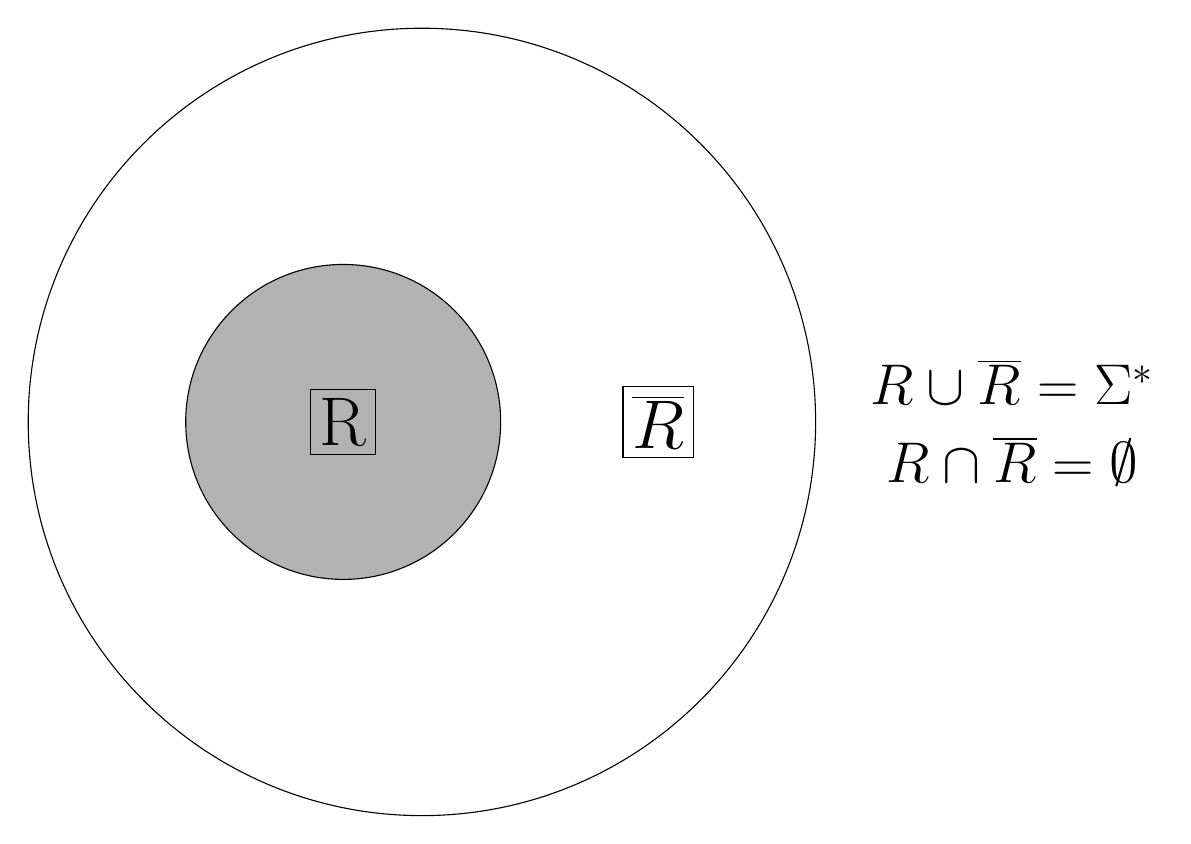
\begin{tikzpicture}
    \filldraw[fill=white, draw=black] (2,2) circle (5cm);
    \node [draw] at (5,2) {\Huge$\overline{R}$};
    \filldraw[fill=gray!60, draw=black] (1,2) circle (2cm);
    \node [draw] at (1,2) {\Huge R};
    \node at (9.5, 2.5) {\huge $R \cup \overline{R} = \Sigma^*$};
    \node at (9.5, 1.5) {\huge $R \cap \overline{R} = \emptyset$};
\end{tikzpicture}}
    \caption{Regular language partition}
    \label{fig:tikz-reg-partition}
\end{figure}

\begin{figure}[!htb]
    \center
    \resizebox{6.5cm}{!}{
    \begin{tikzpicture}
    \usetikzlibrary{calc}
    \node (a) [state] {$R \cup \overline{R} = \top = \Sigma^*$};
    \node (b1) [state, shift={($(a.south)+(1cm, -1cm)$)}] { $R$};
    \node (b2) [state, shift={($(a.south)+(-1cm, -1cm)$)}]{ $\overline{R}$};
    \node (c) [state, shift= {($(a.south) + (0cm, -2.5cm)$)}] { $R \cap \overline{R} = \bot = \emptyset$};
    \draw (a) to (b1);
    \draw (a) to (b2);
    \draw (b1) to (c);
    \draw (b2) to (c);
\end{tikzpicture}}
    \caption{Regular language partition as a lattice}
    \label{fig:tikz-reg-partition-lattice}
\end{figure}

\subsubsection{Abstract tuples}

We define abstract tuples as the product lattice of $\regexs$ and $\uints$ intertwined depending on the schema of the table.
And we define the concretisation function as follows:
\begin{align}
    \concrete_5 &: \bigtimes_{i = 1}^{n}(S_i) \rightarrow \mathcal{P}\left(\bigtimes_{i = 1}^n Z_i \right) \\
    \concrete_5(\ab{e_1}, \ab{e_2}, \dots, \ab{e_n}) &= \concrete_6(\ab{e_1}) \times \concrete_6(\ab{e_2}) \times \dots \times \concrete_6(\ab{e_n})
\end{align}
Where $S_i$ either is $\regexs$ or $\uints$ and $Z_i$ is correspondingly $\strs$ or $\mathbf{NUM}$.

\subsubsection{Single and List values}
When we consider the abstract domain of strings and numbers, we need to consider both single values and lists of values.
We would like to distinguish between single values and lists of values, thus for some set $S$ we define the set $\mathsf{Val} \; S$ inductively as:
\begin{align}
    \inference{}{\bot \in \mathsf{Val} \; S} \quad
    \inference{s \in S}{\mathsf{Single} \; s \in \mathsf{Val} \; S} \quad
    \inference{S' \subseteq S}{\mathsf{List} \; S' \in \mathsf{Val} \; S} \quad
\end{align}
We can define the lattice, $(\mathsf{Val} \; A, \subseteq, \cup, \cap)$, we first define the relation of the lattice:
\begin{align}
    \mathsf{Single} \; s &\sqsubseteq \mathsf{List} \; S \quad
    \text{iff} \; s \in S \\
    \mathsf{Single} \; s_1 &\sqsubseteq \mathsf{Single} \; s_2 \quad
    \text{iff} \; s_1 \sqsubseteq s_2 \\
    \mathsf{List} \; S &\not\sqsubseteq \mathsf{Single} \; s\\
    \mathsf{List} \; S_1 &\sqsubseteq \mathsf{List} \; S_2 \quad
    \text{iff} \; \forall s_1 \in S_1, \; \exists s_2 \in S_2: \; s_1 \sqsubseteq s_2\\
\end{align}

    We define $\cdot \into C_X(S): \ \mathsf{Val} \ S \rightarrow \mathsf{Val} \ C_X(S)$ to be the function that takes some value and inserts it into its cover lattice. \\
    For single elements we use $(\mathsf{Single} \ h) \into C_X(S) = \mathsf{Single}(h\into C_X(S)) \\$
    we say $x \in (\mathsf{Single} \ x') \ \text{iff} \ x = x'.$ \\
    And for a list of elements, we use $(\mathsf{List} \ H) \into C_X(S)=\mathsf{List}(H\into C_X(S))\\$
    we say $x \in (\mathsf{List} \ X) \ \text{iff} \ x \in X.$

We can define the joins and meets of the lattice as follows:
\begin{align}
    \mathsf{Single} \; s \sqcup \mathsf{List} \; S &= \mathsf{List} \; (S\sqcup\left\{ s \right\})\\
    \mathsf{Single} \; s_1 \sqcup \mathsf{Single} \; s_2 &= \mathsf{Single} \; (s \sqcup s )\\
    \mathsf{List} \; S_1 \sqcup \mathsf{List} \; S_2 &= \mathsf{List} \; (S_1 \sqcup S_2)\\
    \mathsf{Single} \; s \sqcap \mathsf{List} \; S &= \mathsf{Single} \; s\\
    \mathsf{List} \; S_1 \sqcap \mathsf{List} \; S_2 &= \mathsf{List} \; (S_1 \sqcap S_2)\\
    \mathsf{Single} \; s_1 \sqcap \mathsf{Single} \; s_2 &= \mathsf{Single} \; (s_1 \sqcap s_2)\\
    \mathsf{List} \ \emptyset \sqcap \mathsf{Single} \ s &= \ \perp
\end{align}
We see that if a list is empty and we look for the meet with a single value, it is equivalent to $\perp$.
As the lattice $(\mathsf{Val} \; A, \subseteq, \cup, \cap)$ is finite, we can use the Kleene fixed-point theorem (see \autoref{thm:kleene_finite}) to prove the termination of our analysis.

We define the concretisation of a variable value as:
\begin{align}
    \concrete_{4a} &: \mathsf{Val} \; \left(C_{X}(S)\right) \rightarrow \mathcal{P}(Z \cup Z^\star) \\
    \concrete_{4a}(\mathsf{Single} \; \ab{s}) &= \concrete_6(\ab{s}) \\
    \concrete_{4a}(\mathsf{List} \; \ab{S'}) &= \bigcup_{n \in \mathbb{N}}\left\{s_1, s_2, \dots, s_n \in Z^n \middle| \forall i \in \{1, 2, \dots, n\} : \exists \ab{s} \in \ab{S'} : s_i \in \concrete_6(\ab{s}) \right\}
\end{align}


\subsubsection{Abstract domain of tables}\label{subsubsec:abstract_domain_of_tables}

We consider a table $t$ as function from the domain of possible tuples in the table $\mathbb{T}$ to the codomain of natural numbers including $0$, $\mathbb{N}$:
\begin{equation}
    t : \mathbb{T} \rightarrow \mathbb{N}.
\end{equation}
The function $t$ describes the number of a given tuple in a table.
We can then consider abstraction over the table $t$ by abstracting either the domain or codomain.
This gives rise to a taxonomy of abstract domains of tables shown in \autoref{tab:taxonomy_of_abstract_domain_of_tables}.
In \autoref{tab:taxonomy_of_abstract_domain_of_tables}, $\mathbb{T}^\#$ denotes an abstract domain of the set of possible tuples $\mathbb{T}$, such that it forms a finite lattice $(\mathbb{T}^\#, \sqsubseteq, \sqcap, \sqcup)$ (and analogous for $\mathbb{N}$).


\begin{table}
    \caption{Taxonomy of abstract domains of tables}
    \centering
    \begin{tabular}{c|l|c}
    Name & Function & Supported \\
    \hline
    \hline
        Bag of tuples & $\mathbb{T} \rightarrow \mathbb{N}$ & \\
        Abstract bag of tuples & $\mathbb{T} \rightarrow \mathbb{N}^\#$ & \\
        Set of tuples & $\mathbb{T} \rightarrow 2$ & \\
        Bag of abstract tuples & $\mathbb{T}^\# \rightarrow \mathbb{N}$ & \\
        Abstract bag of abstract tuples & $\mathbb{T}^\# \rightarrow \mathbb{N}^\#$ & \checkmark \\
        Set of abstract tuples & $\mathbb{T}^\# \rightarrow \{0, some\}$ & \checkmark \\
        Abstract tuple & $\{\cdot\} \rightarrow \mathbb{T}^\#$ & \checkmark \\
    \end{tabular}
    \label{tab:taxonomy_of_abstract_domain_of_tables}
\end{table}

We will only consider abstract bags of abstract tuples, sets of abstract tuples and abstract tuples because of their finite nature.
It should be clear that sets of abstract tuples are just a special case of abstract bags of abstract tuples.
Naturally, these maps all form map lattices.

We define the concretisation of a table as:
\begin{align}
    \concrete_{4d} &: \mathcal{P}\left(\bigtimes_{i = 1}^{n}S_i\right) \rightarrow \mathcal{M}\left(\bigtimes_{i = 1}^n Z_i\right) \\
    \concrete_{4d}(\ab{t}) &= \left\{ t \in \mathcal{M}\left(\bigtimes_{i = 1}^n Z_i\right) \middle|\forall e \in t : \exists \ab{e} \in \ab{t} : e \in \concrete_5(\ab{e}) \right\}
\end{align}

\subsubsection{Abstract environments}

We define an abstract environment $\rho_{\ab{a}} \in \ab{\mathfrak{E}_a}$ mapping application variable names $v_a \in \mathbb{V}_a$ to abstract values, and $\rho_{\ab{d}} \in \ab{\mathfrak{E}_d}$ mapping table names $v_d \in \mathbb{V}_d$ to abstract tables, in symbols:
\begin{align}
    \ab{\mathfrak{E}_a} &= \mathbb{V}_a \rightarrow \mathsf{Val} \; (\regexs) \cup \mathsf{Val} \; (\uints) \\
    \ab{\mathfrak{E}_d} &= \mathbb{V}_d \rightarrow \regexs \cup \uints \cup \regexs \times \regexs \cup \regexs \times \uints \dots \\
    \ab{\mathfrak{E}} &= \ab{\mathfrak{E}_a} \times \ab{\mathfrak{E}_d}
\end{align}

Naturally we define the concretisation functions for environments as:
\begin{align}
    \concrete_2 &: \ab{\mathfrak{E}} \rightarrow \mathcal{P}(\mathfrak{E}) \\
    \concrete_2(\rho_{\ab{d}}, \rho_{\ab{a}}) &= \concrete_{3d}(\rho_{\ab{d}}) \times \concrete_{3a}(\rho_{\ab{a}})
\end{align}
\begin{align}
    \concrete_{3d} &: \ab{\mathfrak{E}_d} \rightarrow \mathcal{P}(\mathfrak{E}_d) \\
    \concrete_{3d}(\rho_{\ab{d}}) &= \left\{ \rho_{a} \in \mathfrak{E}_d \middle| \forall v_d \in \mathbb{V}_d : \rho_d(v_d) \in \concrete_{4d}(\rho_{\ab{d}}(v_d)) \right\}
\end{align}
\begin{align}
    \concrete_{3a} &: \ab{\mathfrak{E}_a} \rightarrow \mathcal{P}(\mathfrak{E}_a) \\
    \concrete_{3a}(\rho_{\ab{a}}) &= \left\{ \rho_{a} \in \mathfrak{E}_a \middle| \forall v_a \in \mathbb{V}_a : \rho_a(v_a) \in \concrete_{4a}(\rho_{\ab{a}}(v_a)) \right\}
\end{align}
And in the same vain we define a concretisation function for sets of environments as:
\begin{align}
    \concrete_1 &: \mathcal{P}(\ab{\mathfrak{E}}) \rightarrow \mathcal{P}(\mathfrak{E}) \\
    \concrete_1(\ab{P}) &= \left\{ (\rho_{d}, \rho_{a}) \in \mathfrak{E} \middle| \exists (\rho_{\ab{d}}, \rho_{\ab{a}}) \in \ab{P} : (\rho_{d}, \rho_{a}) \in \concrete_2(\rho_{\ab{d}}, \rho_{\ab{a}})\right\}
\end{align}

